\section{Linear regression by several forms}
\subsection{Closed Form}

\begin{listing}[H]
    \begin{minted}[frame=lines, breaklines, breaksymbolleft=, fontsize=\footnotesize]{python}
def linReg(X, y):
    weights = np.linalg.inv(X.T @ X) @ X.T @ y
    preds = X @ weights
    return preds, weights
    \end{minted}
\end{listing}

\subsection{Gradient Descent}

\begin{listing}[H]
    \begin{minted}[frame=lines, breaklines, breaksymbolleft=, fontsize=\footnotesize]{python}
def linRegGD(X, y, iters, l=0.00001):
    weights = np.zeros((features, 1))
    
    iterations = np.empty(iters)
    for i in range(iters):
        update = 2 * X.T @ ((X @ weights) - y)
        weights = weights - l * update
        iterations[i] = np.linalg.norm(y - X @ weights)
    
    preds = X @ weights
    return preds, weights, iterations
    \end{minted}
\end{listing}

\subsection{Stochastic Gradient Descent}

\begin{listing}[H]
    \begin{minted}[frame=lines, breaklines, breaksymbolleft=, fontsize=\footnotesize]{python}
def linRegSGD(X, y, iters, l=0.05):
    weights = np.zeros((X.shape[1], 1))
    iterations = np.empty(iters)
    
    for i in range(iters):  
        j = np.floor(np.random.rand()*X.shape[0]).astype(int)
        error = (X[j] @ weights) - y[j]
        update = error * X[j].T
        weights = weights - l * update.reshape(update.shape[0], 1)
      
        iterations[i] = np.linalg.norm(X @ weights - y)
        
    preds = X @ weights
    return preds, weights, iterations
    \end{minted}
\end{listing}

\subsection{Comparisons}
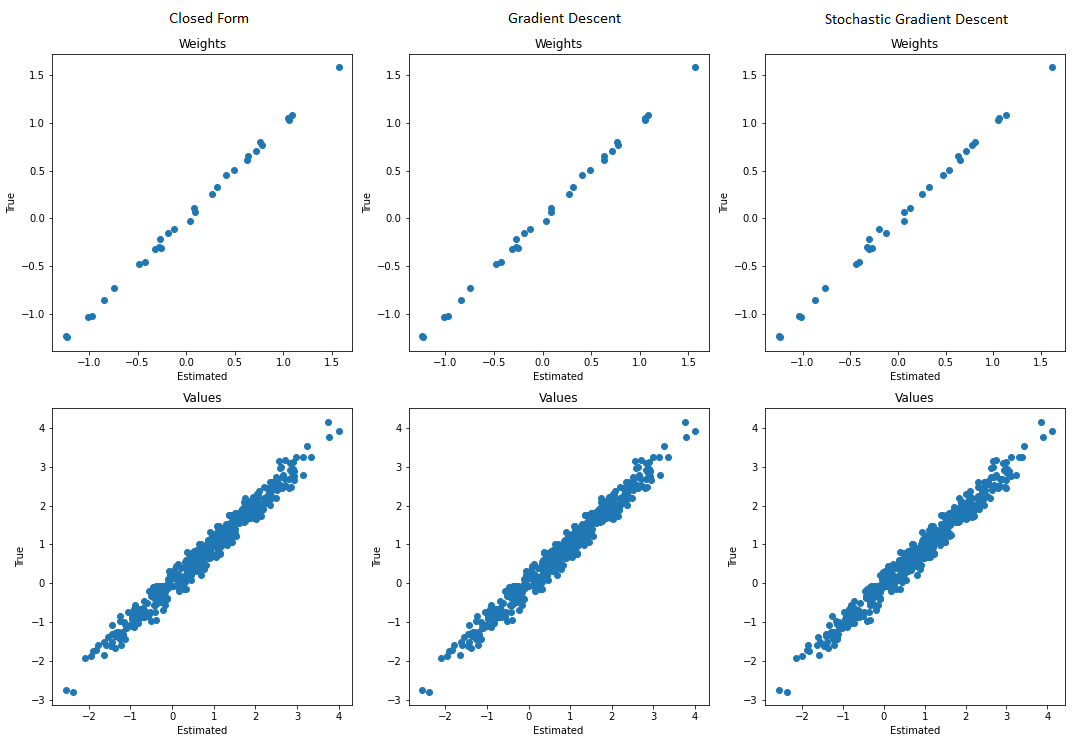
\includegraphics[width=\linewidth]{figs/LinRegComparison.png}
To put a numerical figure on the accuracy of learning between these methods, I compared the true weights of the data to the weights that were found by each method using MSE. 
\begin{center}
    \begin{tabular}{| c c |}
        \hline
        Algorithm & Weight MSE \\ 
        \hline\hline
        Closed Form & $7.298 \times 10^{-4}$\\ 
        Gradient Descent & $7.294 \times 10^{-4}$ \\
        Stochastic Gradient Descent & $1.900 \times 10^{-3}$\\
        \hline      
    \end{tabular}
\end{center}
With careful tuning, the weights MSE between closed form and gradient descent were brought to within 0.05\% of each other. 
This shows how the closed form method and gradient descent are the most accurate at replicating the true weights, although this requires delicate tuning to get the performance in GD. Stochastic Gradient Descent follows these methods by a factor of 10.

Gradient Descent over the whole dataset provides a very smooth error graph. By effectively averaging the update that needs to be done for every data point and using this to update the weights provides a much smoother descent to the minimum.
Stochastic Gradient Descent on the other hand is very fuzzy and not well defined, the loss has iterations where it will increase instead of decrease which means it can be uncertain when to stop. This is due to the single sample nature of this algorithm, by updating the weights using only a single sample the change may not capture the entire dataset and result in a net loss of accuracy.
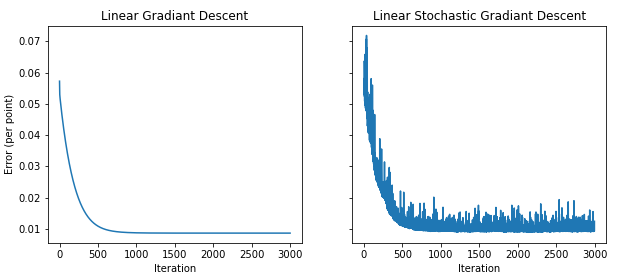
\includegraphics[width=\linewidth]{figs/GD vs SGD.png}
As a result of the fuzzy nature of Stochastic Gradient Descent the final error of the algorithm is not quite as low as Gradient Descent. 
\subsection{Improving SGD}
To combat the issue of jumping loss within SGD I implemented a technique where the learning rate is lowered proportionally to the iteration through the dataset. By gradually lowering the learning rate in this fashion the steps the algorithm takes when updating the weights gets lower and lower, eventually converging on to the local minima instead of jumping around a value.
\begin{listing}[H]
    \begin{minted}[frame=lines, breaklines, breaksymbolleft=, fontsize=\footnotesize]{python}
def linRegSGD_smoothed(X, y, iters, lb=0.05, le=None):
    if(le==None):
        le = lb/10
    weights = np.zeros((X.shape[1], 1))
    #decrease learning rate through iterations
    l = np.linspace(lb,le,iters)
    iterations = np.empty(iters)
    
    for i in range(iters):  
        j = np.floor(np.random.rand()*X.shape[0]).astype(int)
        update = ((X[j] @ weights) - y[j]) * X[j].T
        weights = weights - l[i] * update.reshape(update.shape[0], 1)
      
        iterations[i] = np.linalg.norm(X @ weights - y)
        
    preds = X @ weights
    return preds, weights, iterations
    \end{minted}
\end{listing}
This succeeds in smoothing the error across iterations within SGD, but at the detriment of further increasing the error score of this algorithm at the end of iterations.

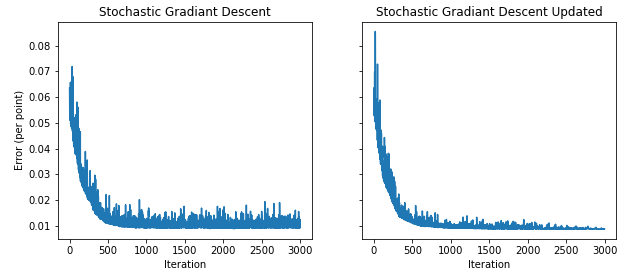
\includegraphics[width=\linewidth]{figs/SGDFixed.png}

